%! TEX root = ../main.tex
% ==============================================================
% IMMUTABLE — generated automatically, do not edit this block
%
% — Provenance ───────────────────────────────────────────────────
%   script            : analysis_scratch/peaktrough_vs_fft_demo_cropped.py
%   computed_in       : analysis_scratch/peaktrough_vs_fft_demo_cropped.py (per-freq IN-probe time-series render)
%   plot_type         : amp_methods_demo
%   data_class        : DELEG
%   generated_at      : 2026-05-07T10:58:44
%   findings_doc      : memory/methodology_window_mean_baseline.md
%
% — Thesis context ──────────────────────────────────────────────
%   chapter           : 04
%   caption_label     : fig:ch04_amp_methods_a1_fullwind
%   caption_short     : Tre amplitudemetoder, $A_1$ med vind
%
% — Filters ────────────────────────────────────────────────────
%   panel             : full
%   wind              : full
%   amplitude [V]     : 0.1
%   frequency [Hz]    : 1.3, 1.4, 1.5, 1.6
%   probes            : 
%   run_category      : 
%   quality_flag      : ok
%   mooring           : 
%
% — Data provenance ────────────────────────────────────────────
%   n_runs            : 
%   in_probes_used    : 
%   out_probes_used   : 
%   probe_configs     : 
%   non_final_config_n: 
%   datasets        :
%     PROCESSED-20251005-sixttry6roof-highMooring
%     PROCESSED-20251110-tett6roof-lowMooring
%     PROCESSED-20251110-tett6roof-lowMooring-2
%     PROCESSED-20251112-tett6roof
%     PROCESSED-20251113-tett6roof
%     PROCESSED-20251113-tett6roof-loosepaneltaped
%     PROCESSED-20251113-tett6roof-probeadjusted
%     PROCESSED-20260305-newProbePos-tett6roof
%     PROCESSED-20260306-newProbePos-tett6roof
%     PROCESSED-20260307-ProbPos4_31_FPV_2-tett6roof
%     PROCESSED-20260312-ProbPos4_31_FPV_2-tett6roof
%     PROCESSED-20260313-ProbePos4_31_FPV_2-tett6roof
%     PROCESSED-20260314-ProbePos4_31_FPV_2-tett6roof
%     PROCESSED-20260316-ProbePos4_31_FPV_2-tett6roof
%     PROCESSED-20260316-ProbePos4_31_FPV_2-tett6roof-under9Mooring
%     PROCESSED-20260319-ProbePos4_31_FPV_2-tett6roof-under9Mooring
%     PROCESSED-20260321-ProbePos4_31_FPV_2-tett6roof-under9Mooring-height100-RENAMED
%     PROCESSED-20260323-ProbePos4_31_FPV_2-tett6roof-under9Mooring-height100
%     PROCESSED-20260323-ProbePos4_31_FPV_2-tett6roof-under9Mooring-height136
%     PROCESSED-20260324-ProbePos4_31_FPV_2-tett6roof-under9Mooring-height100
%     PROCESSED-20260325-ProbePos4_31_FPV_2-tett6roof-under9Mooring-height100
%     PROCESSED-20260326-ProbePos4_31_FPV_2-tett6roof-under9Mooring-height100
%     PROCESSED-20260326-ProbePos4_31_FPV_2-tett6roof-under9Mooring-height100-lowrange
%     PROCESSED-20260327-ProbePos4_31_FPV_2-tett6roof-under9Mooring30-height100-lowrange
%   run_paths       :
%     (omitted — aggregate over > threshold runs, see datasets)
%
% — Method / numerical parameters ─────────────────────────────
%   grouper           : 
%   collapse_panels   : 
%   fft_window_hz     : 0.1
%   extra_params      : runs=4 (1.3/1.4/1.5/1.6 Hz, fullpanel/fullwind/A_1/per240/mstop30, canon dataset 20260327-...lowrange). probe=IN:9373/170 only. display window = absolute [23.20, 28.20] s (x-axis shows absolute recording time, 'fra start'). per-panel amplitude values (A_FFT, A_p, A_phi) are pulled from each run's meta.json — computed over each run's own 10-period analysis window (Computed Probe 9373/170 start/end), NOT over the visible 5 s slice. A_FFT = nearest-bin FFT magnitude at f_paddle (0.1 Hz half-window). A_p   = (P99.5 − P0.5)/2 over the analysis window. A_phi = mean of |signed| samples at u+T/4 and u+3T/4 across the detected upcrossings inside the analysis window. Bands: ±A_FFT (solid green), ±A_p (dashed red), ±A_phi (dotted blue). Per-panel value legend above the axis shows marker + value + percent inflation vs A_FFT. f badge in upper-right corner. Typeset in NewComputerModern10 to match thesis body font.
%
% — Summary stats cited in caption ────────────────────────────
%   stat:f13_A_FFT_mm : 7.484
%   stat:f13_A_p_mm   : 13.993
%   stat:f13_A_phi_mm : 5.086
%   stat:f13_p_inflate_pct : 87.0
%   stat:f13_phi_inflate_pct : -32.0
%   stat:f13_window_abs_s : [20.916, 28.596]
%   stat:f13_phi_n_cycles : 16
%   stat:f14_A_FFT_mm : 7.710
%   stat:f14_A_p_mm   : 11.482
%   stat:f14_A_phi_mm : 6.651
%   stat:f14_p_inflate_pct : 48.9
%   stat:f14_phi_inflate_pct : -13.7
%   stat:f14_window_abs_s : [22.084, 29.244]
%   stat:f14_phi_n_cycles : 11
%   stat:f15_A_FFT_mm : 9.181
%   stat:f15_A_p_mm   : 13.606
%   stat:f15_A_phi_mm : 7.674
%   stat:f15_p_inflate_pct : 48.2
%   stat:f15_phi_inflate_pct : -16.4
%   stat:f15_window_abs_s : [22.372, 29.052]
%   stat:f15_phi_n_cycles : 10
%   stat:f16_A_FFT_mm : 9.151
%   stat:f16_A_p_mm   : 14.322
%   stat:f16_A_phi_mm : 8.269
%   stat:f16_p_inflate_pct : 56.5
%   stat:f16_phi_inflate_pct : -9.6
%   stat:f16_window_abs_s : [23.324, 29.588]
%   stat:f16_phi_n_cycles : 10
%   stat:display_window_abs_s : [23.20, 28.20]
%   stat:probe        : 9373/170
%   stat:amp_input_V  : 0.10
%   stat:wind_condition : fullwind
%   stat:sampling_rate_Hz : 250.0
%
% — Subfigures available ───────────────────────────────────────
%     FIGURES/ch04_amp_methods_a1_fullwind.pdf
% ── end immutable block ─────────────────────────────────────────
\begin{figure}[htbp]
  \centering
  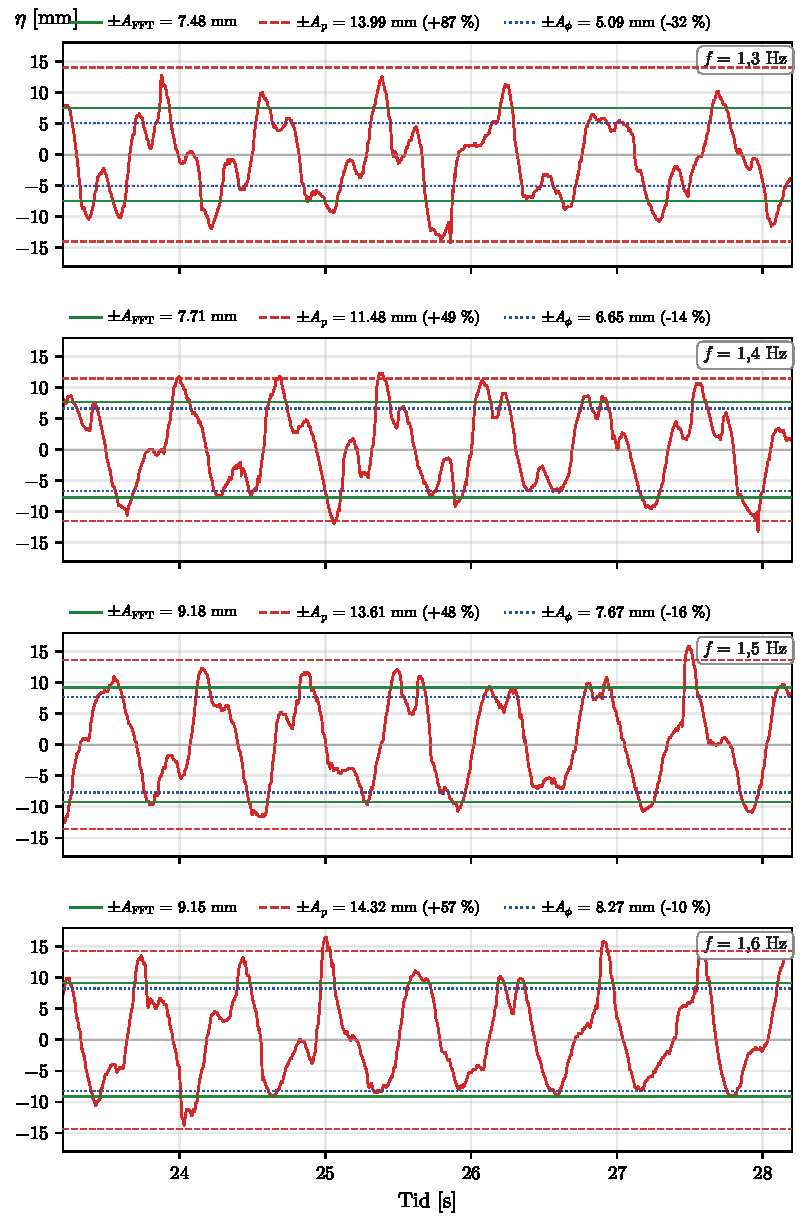
\includegraphics[width=\linewidth]{FIGURES/ch04_amp_methods_a1_fullwind.pdf}
  \caption[Tre amplitudemetoder, $A_1$ med vind]{
    Nærbilde av tidsserier for innkommende bølge, $A_1$. Full vind for alle fire frekevensene. Samme tidsakse i sekunder fra start.  Verdiene er beregnet fra hver bølges eget vindu på 10 perioder.
  }
  \label{fig:ch04_amp_methods_a1_fullwind}
\end{figure}
